\documentclass[12]{article}

%Spell Check
\usepackage[british]{babel}

% Header & Footer
\usepackage{lipsum}
\usepackage{geometry}
\usepackage{fancyhdr}
\usepackage{charter}

% Bibliograhpy
\usepackage[super,numbers,sort&compress]{natbib}

%Image Software
\usepackage{graphicx}
\usepackage[space]{grffile}
\usepackage{float}

%Equation Software
\usepackage{bm}

\pagestyle{fancy}
\fancyhead{}
\fancyfoot{}
\fancyhead[R]{Page \thepage}
\renewcommand{\headrulewidth}{0.5pt}
\renewcommand{\footrulewidth}{0.5pt}

\begin{document}
\begin{titlepage}
\begin{center}
	
	\LARGE{\bf{Tobor Inc Automation Process}}\\
	[1cm]
	\large{J. R. Harper \\ QA Consulting \\ Project Supervisor: Roberto Fernandez}\\
	\large{Chris Lucas: Consultant Project Liason } \\
	[0.2cm]
	\line(1,0){400} \\
	
\end{center}


\end{titlepage}

\cleardoublepage

\tableofcontents

\thispagestyle{empty}
\pagenumbering{arabic}

\cleardoublepage

%First page

\section{Introduction}\label{sec:intro}

I have been contracted to help Tobor Inc. automate their content aggregation service. This is under the project manager Roberto Fernandez, the Project Liaison Chris Lucas and the Managing Director David Bradbury. 
\\
The services to be automated included the user registration service, the content aggregation, and lastly sending a report of all actions to Tobor Inc. With regards to registration, this includes any new users, any updates that may need to happen to their accounts, or lastly if they wish for an account deletion.
\\
The content aggregated is to be from three separate websites at minimum, and to be formatted in such a way to be easily readable by the user who has signed up for the service. There is also need for different content types to be collected, those being sport, tech or hobbies. 
\\
Finally, the report is to include any user changes, the content collected and the users who received the content formatted.

\setcounter{page}{1}

\section{State of Project}

As it stands, all the process listed are performed manually by Roberto and his team. The aim is to have all of these automated to free their workload within Tobor.

\begin{figure}[H]
	\centering
	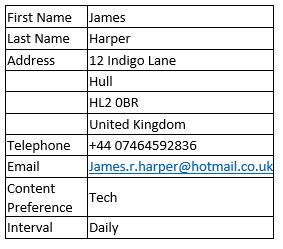
\includegraphics[height=1.5in]{C:/Users/james/Documents/Work/QA Consulting/Training Notes/Project (5 - 9)/Documentation/Images/Email Table}
	\caption{Table used for registration}
	\label{fig:RegistrationTable}
\end{figure}

As was seen in figure \ref{fig:RegistrationTable} Tobor Inc. started out with using a HTML table sent through an email. This has now been adpapted for automation use with each box having an index of zero through to twenty, with the properties tables being zero, two, four etc... and the information being one, three, five etc... These tables can now be used as the standard format, as before, but with the robot calling the required index.

\begin{figure}[H]
	\centering
	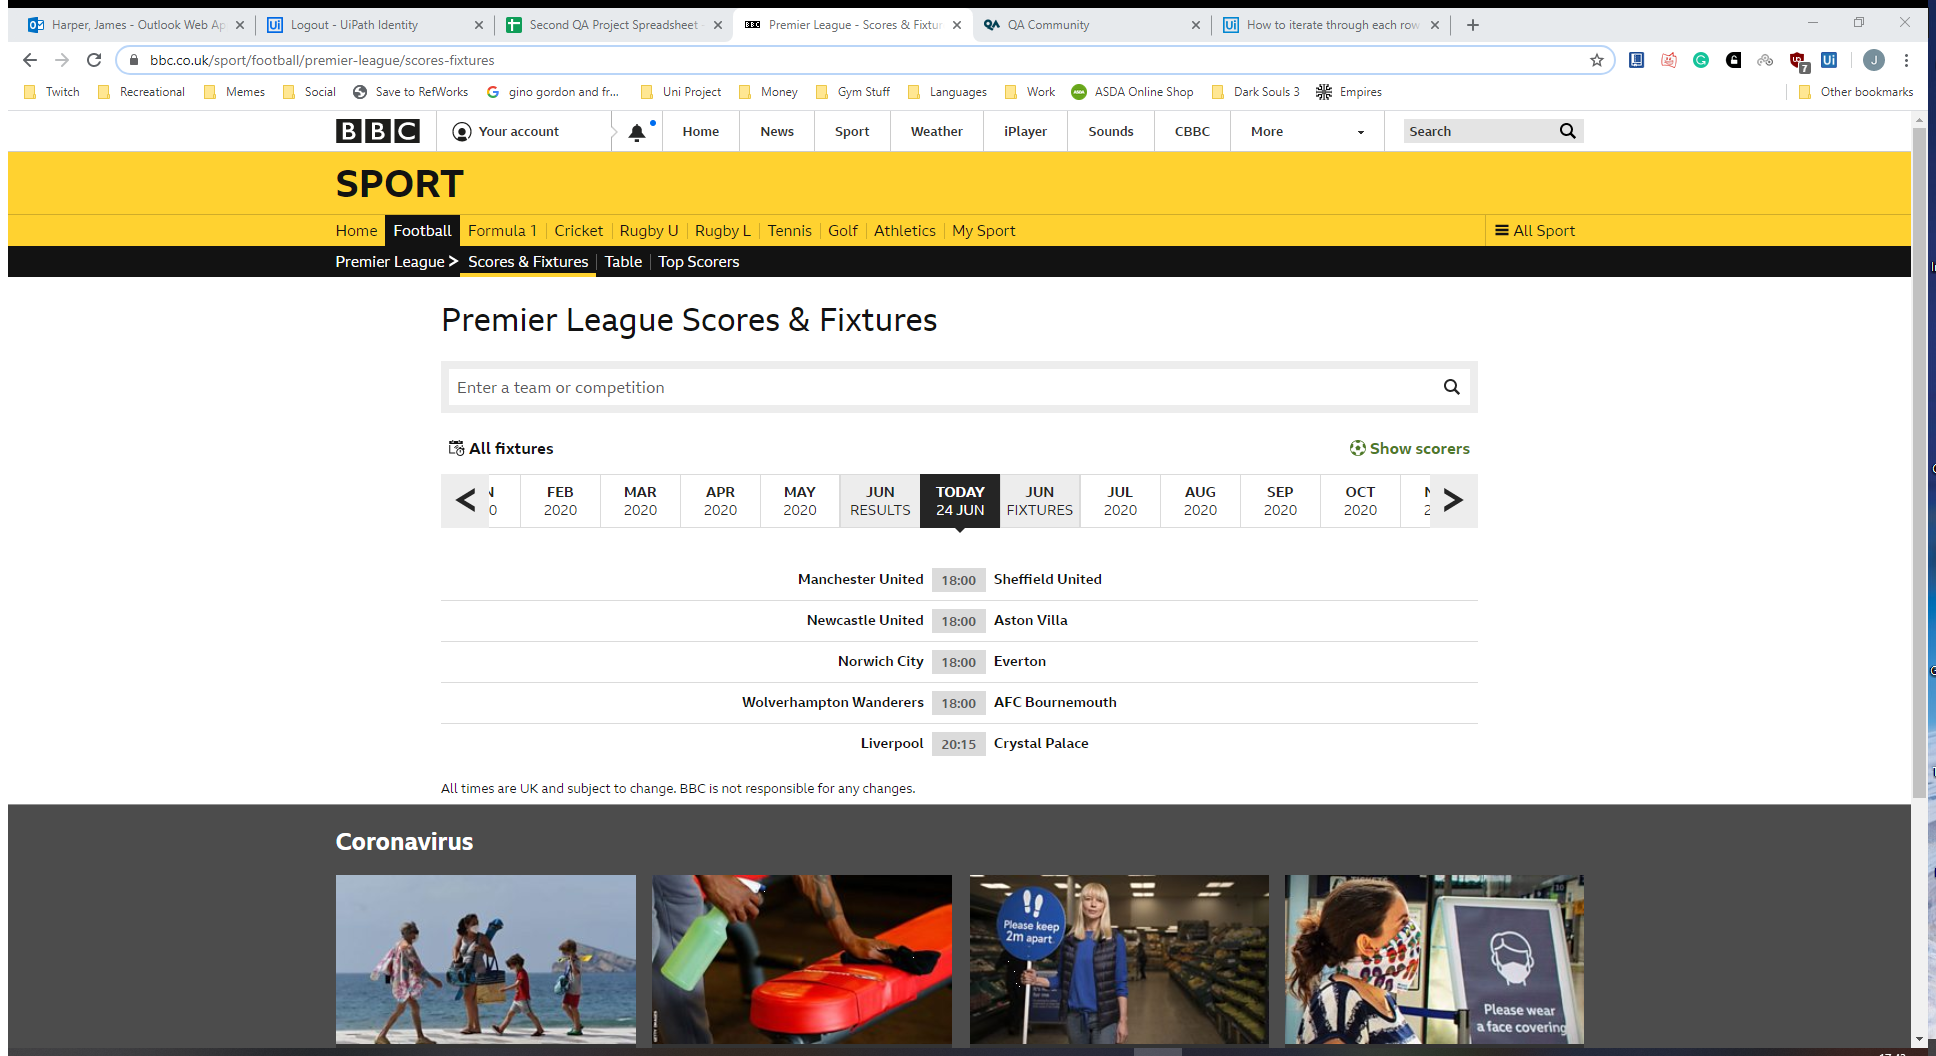
\includegraphics[height=2in]{C:/Users/james/Documents/Work/QA Consulting/Training Notes/Project (5 - 9)/Documentation/Images/BBC Sports Table}
	\caption{Example Page that was scanned}
	\label{fig:BBCSport}
\end{figure}

\begin{figure}[H]
	\centering
	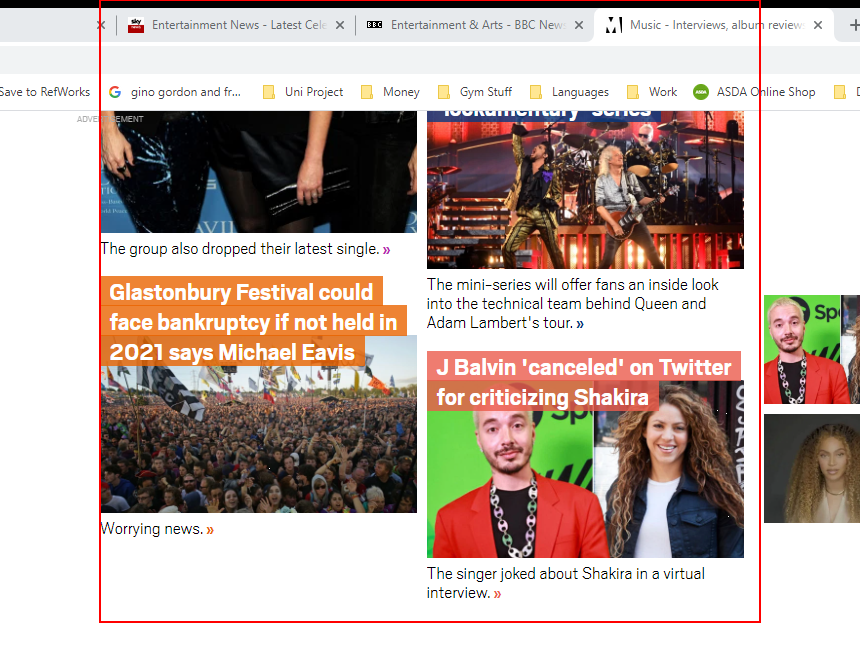
\includegraphics[height=2in]{C:/Users/james/Documents/Work/QA Consulting/Training Notes/Project (5 - 9)/Documentation/Images/News Highlighted}
	\caption{Second example Page that was scanned}
	\label{fig:Scan}
\end{figure}

Figure \ref{fig:BBCSport} and \ref{fig:Scan} show example pages that were scanned by UIPath. Both demonstrate the process used to pick up data and the thought process that went behind choosing the websites. This is shown by using websites that had tabular data, making for easier pick ups by UIPath. This enables not only an easier report collection as this can then be stacked into a secondary table per piece of news reported, but also allows for easier email formatting, enabling a smoother content delivery.

\begin{figure}[H]
	\centering
	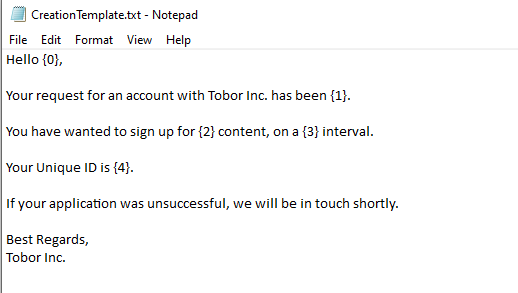
\includegraphics[height=2in]{C:/Users/james/Documents/Work/QA Consulting/Training Notes/Project (5 - 9)/Documentation/Images/Email Template}
	\caption{Example of an email template used}
	\label{fig:EmailTemplate}
\end{figure}

Figure \ref{fig:EmailTemplate} is one of the many email templates that have been set up for this automation. They have been created with the intent of speeding content delivery for the user and to provide an easily formattable environment for not only the RPA maintainer to go through, but it also allows for a clearer detail delivery to the user.

\begin{figure}[H]
	\centering
	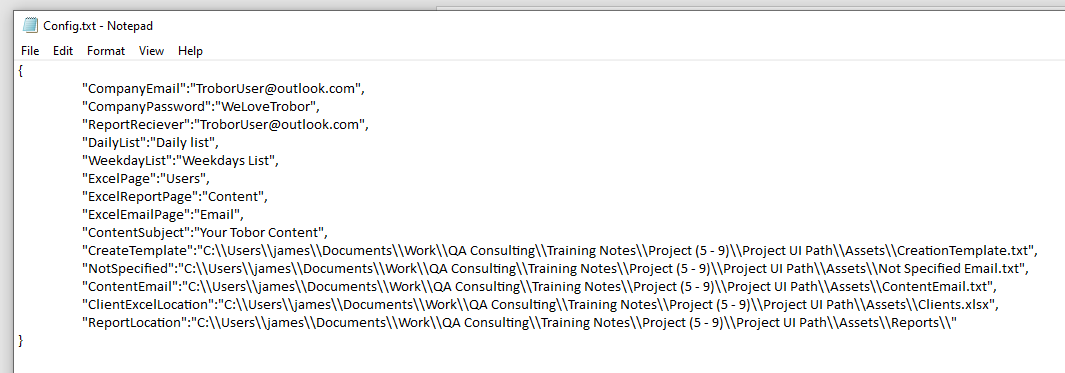
\includegraphics[height=1.5in]{C:/Users/james/Documents/Work/QA Consulting/Training Notes/Project (5 - 9)/Documentation/Images/Config}
	\caption{Example of a config file used}
	\label{fig:Config}
\end{figure}

Figure \ref{fig:Config} can show how the RPA solutions developed can be intended for long term use, and not just while they have an active developer on the site. Config files such as this help enable the company to maintain the program without having to a) have a knowledge of UIPath, and b) go inside of the UIPath application. 

\begin{figure}[H]
	\centering
	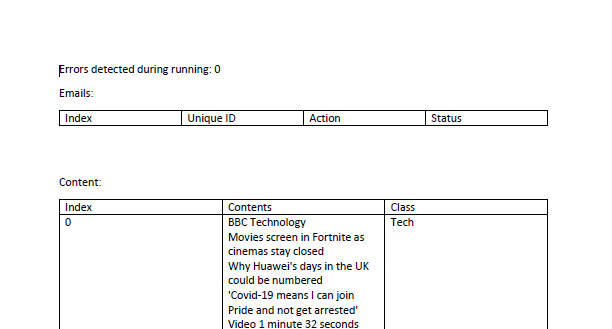
\includegraphics[height=1.5in]{C:/Users/james/Documents/Work/QA Consulting/Training Notes/Project (5 - 9)/Documentation/Images/Report Part One}
	\caption{Part one of an example report .pdf}
	\label{fig:ReportOne}
\end{figure}

\begin{figure}[H]
	\centering
	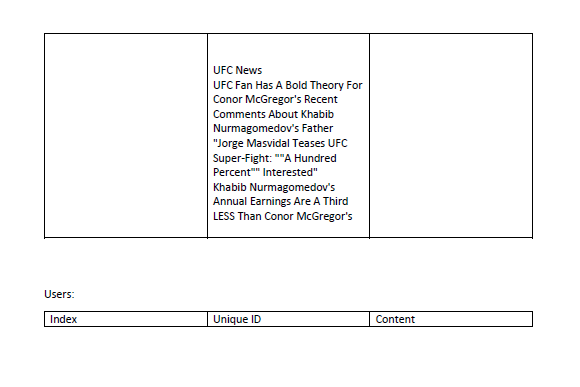
\includegraphics[height=1.5in]{C:/Users/james/Documents/Work/QA Consulting/Training Notes/Project (5 - 9)/Documentation/Images/Report Part Two}
	\caption{Part two of an example report .pdf}
	\label{fig:ReportTwo}
\end{figure}

Both figures \ref{fig:ReportOne} and \ref{fig:ReportTwo} show the result of the report output. This can now be automatically done by the program, and allows for a consistent keeping of records, unlike prior to the automation.

\section{Benefits}

\begin{table}[H]
\centering
\begin{tabular}{|l|l|}
\hline
Step                & Time Consumed (m) \\ \hline
New Registration    & 15 per user       \\
Content Aggregation & 120               \\
Content Send Off    & 10                \\
Report Collating    & 15 per user       \\
                    &                  
\end{tabular}
\end{table}

As discussed in the prior chapters, the enabling of automation helps Tobor Inc. reduce the time investment by their staff. This can be summarised by the table seen. The usual daily users that were requesting content could be up to and around 50 people, which as seen by the table means a lot of time was used, hence the introduction of the automated process.

In addition, allowing staff to work on other areas of the business instead of collating this data means that Tobor Inc. will have an excess of resources available for other areas of the business.

\section{Challenges}

Unfortunately, automating a series of tasks such as these can come with its own issues. For example, if a website changes their layout, any of the files get corrupted or change location, or even if the program is moved to a cloud resource instead of being hosted locally. Luckily, these are all address in the risk assessment given within this document.


\end{document}